\documentclass[../Matt_Gebert_Honours_Thesis.tex]{subfiles}

\begin{document}
% I describe the various ways of producing and identifying graphene in lab use, and the characterisations I have conducted. This will include our use of atomic force microscopy (AFM), optical microscopy and Raman spectroscopy.

\section{Raman spectroscopy}

Raman spectroscopy uses monochromatic light to observe scattering processes on an incident material. Four fundamental processes describe the scattering behaviour: IR absorption, Rayleigh scattering, or (anti) Stokes Raman scattering. The latter (two) processes scatter light, by interactions with phonons or other excitations. This changes the incident light's momentum and energy, resulting in a frequency shift. By measuring the returning light and it's spectral distribution, information is gained of the vibrational modes within the material. Devices such as charged coupled devices (using MOS or CMOS transistors) allow for sensitive measurements of the light across different frequencies. Photons that are scattered with the same initial energy (Rayleigh Scattering) are filtered.

\subsection{Raman in graphite}
Historically, the Raman profile for graphite is well established \cite{vidano_observation_1981}. Since the invention of the laser to make sensitive, monochromatic measurements, Raman spectroscopy conducted in the 1970's had yielded a distinct profile of the phonons existing within  graphite\cite{nemanich_first-_1979,tuinstra_characterization_1970,tuinstra_raman_1970}. At the beginning of the 80's Vidano's group profiled graphite samples across multiple Raman wavelengths, properly profiling different peaks \cite{vidano_observation_1981}. 

Peaks are listed as follows:
\begin{itemize}[noitemsep,topsep=0pt,leftmargin=0.4cm]
	\item \textbf{G} ($\approx$1580/cm)\hspace{0.2cm}The active $2E_{2g}$ mode of the hexagonal symmetry group. This traditionally has the highest peak intensity in graphite, and is doubly degenerate.
	\item \textbf{2D} ($\approx$2700/cm)\hspace{0.2cm}Higher order scattering, and overtone of D. Second highest peak in graphite. Relabelled as the 2D peak by Ferrari, originally written as G' peak.
	\item \textbf{D} ($\approx$1360/cm)\hspace{0.2cm}Attributed to edge modes (ie zone boundaries) that appear from relaxed wavevector selection rules.
	\item \textbf{D'} ($\approx$1620/cm)\hspace{0.2cm}Splitting from degenerate $E_{2g}$ due to disorder.
	\item \textbf{D''} ($\approx$2950/cm)\hspace{0.2cm}Higher order scattering.	
\end{itemize}
In graphite, the G peak is normally dominant and the 2D peak is split into at least two components at $1/2$ and $1/4$ amplitudes of the G peak. 

\subsection{Raman in graphene}
Differing layer numbers of graphene produce unique Raman signals\cite{ferrari_raman_2006,ferrari_raman_2013}. This variance in the amplitude and central frequency of maxima. The signals are unique because the vibrational and electronic properties of monolayer, bilayer and multilayer are distinct. Ferrari \etal{}. observed that Raman is a useful tool for distinguishing between these layers.

Two particular characteristics are useful for characterising layers. Firstly the amplitude of the 2D peak is roughly on the order of 2x that of the G peak in graphene. This ratio drops as the number of layers increases. Only the single layer and bilayer peaks are easily distinct from higher numbers of layers, which are somewhat indistinguishable.

This characteristic is clear in the data aquired of numerous graphene samples shown below in \cref{fig:raman_data_1}.
\begin{figure}[H]
%	\begin{subfigure}{0.3\textwidth}
%		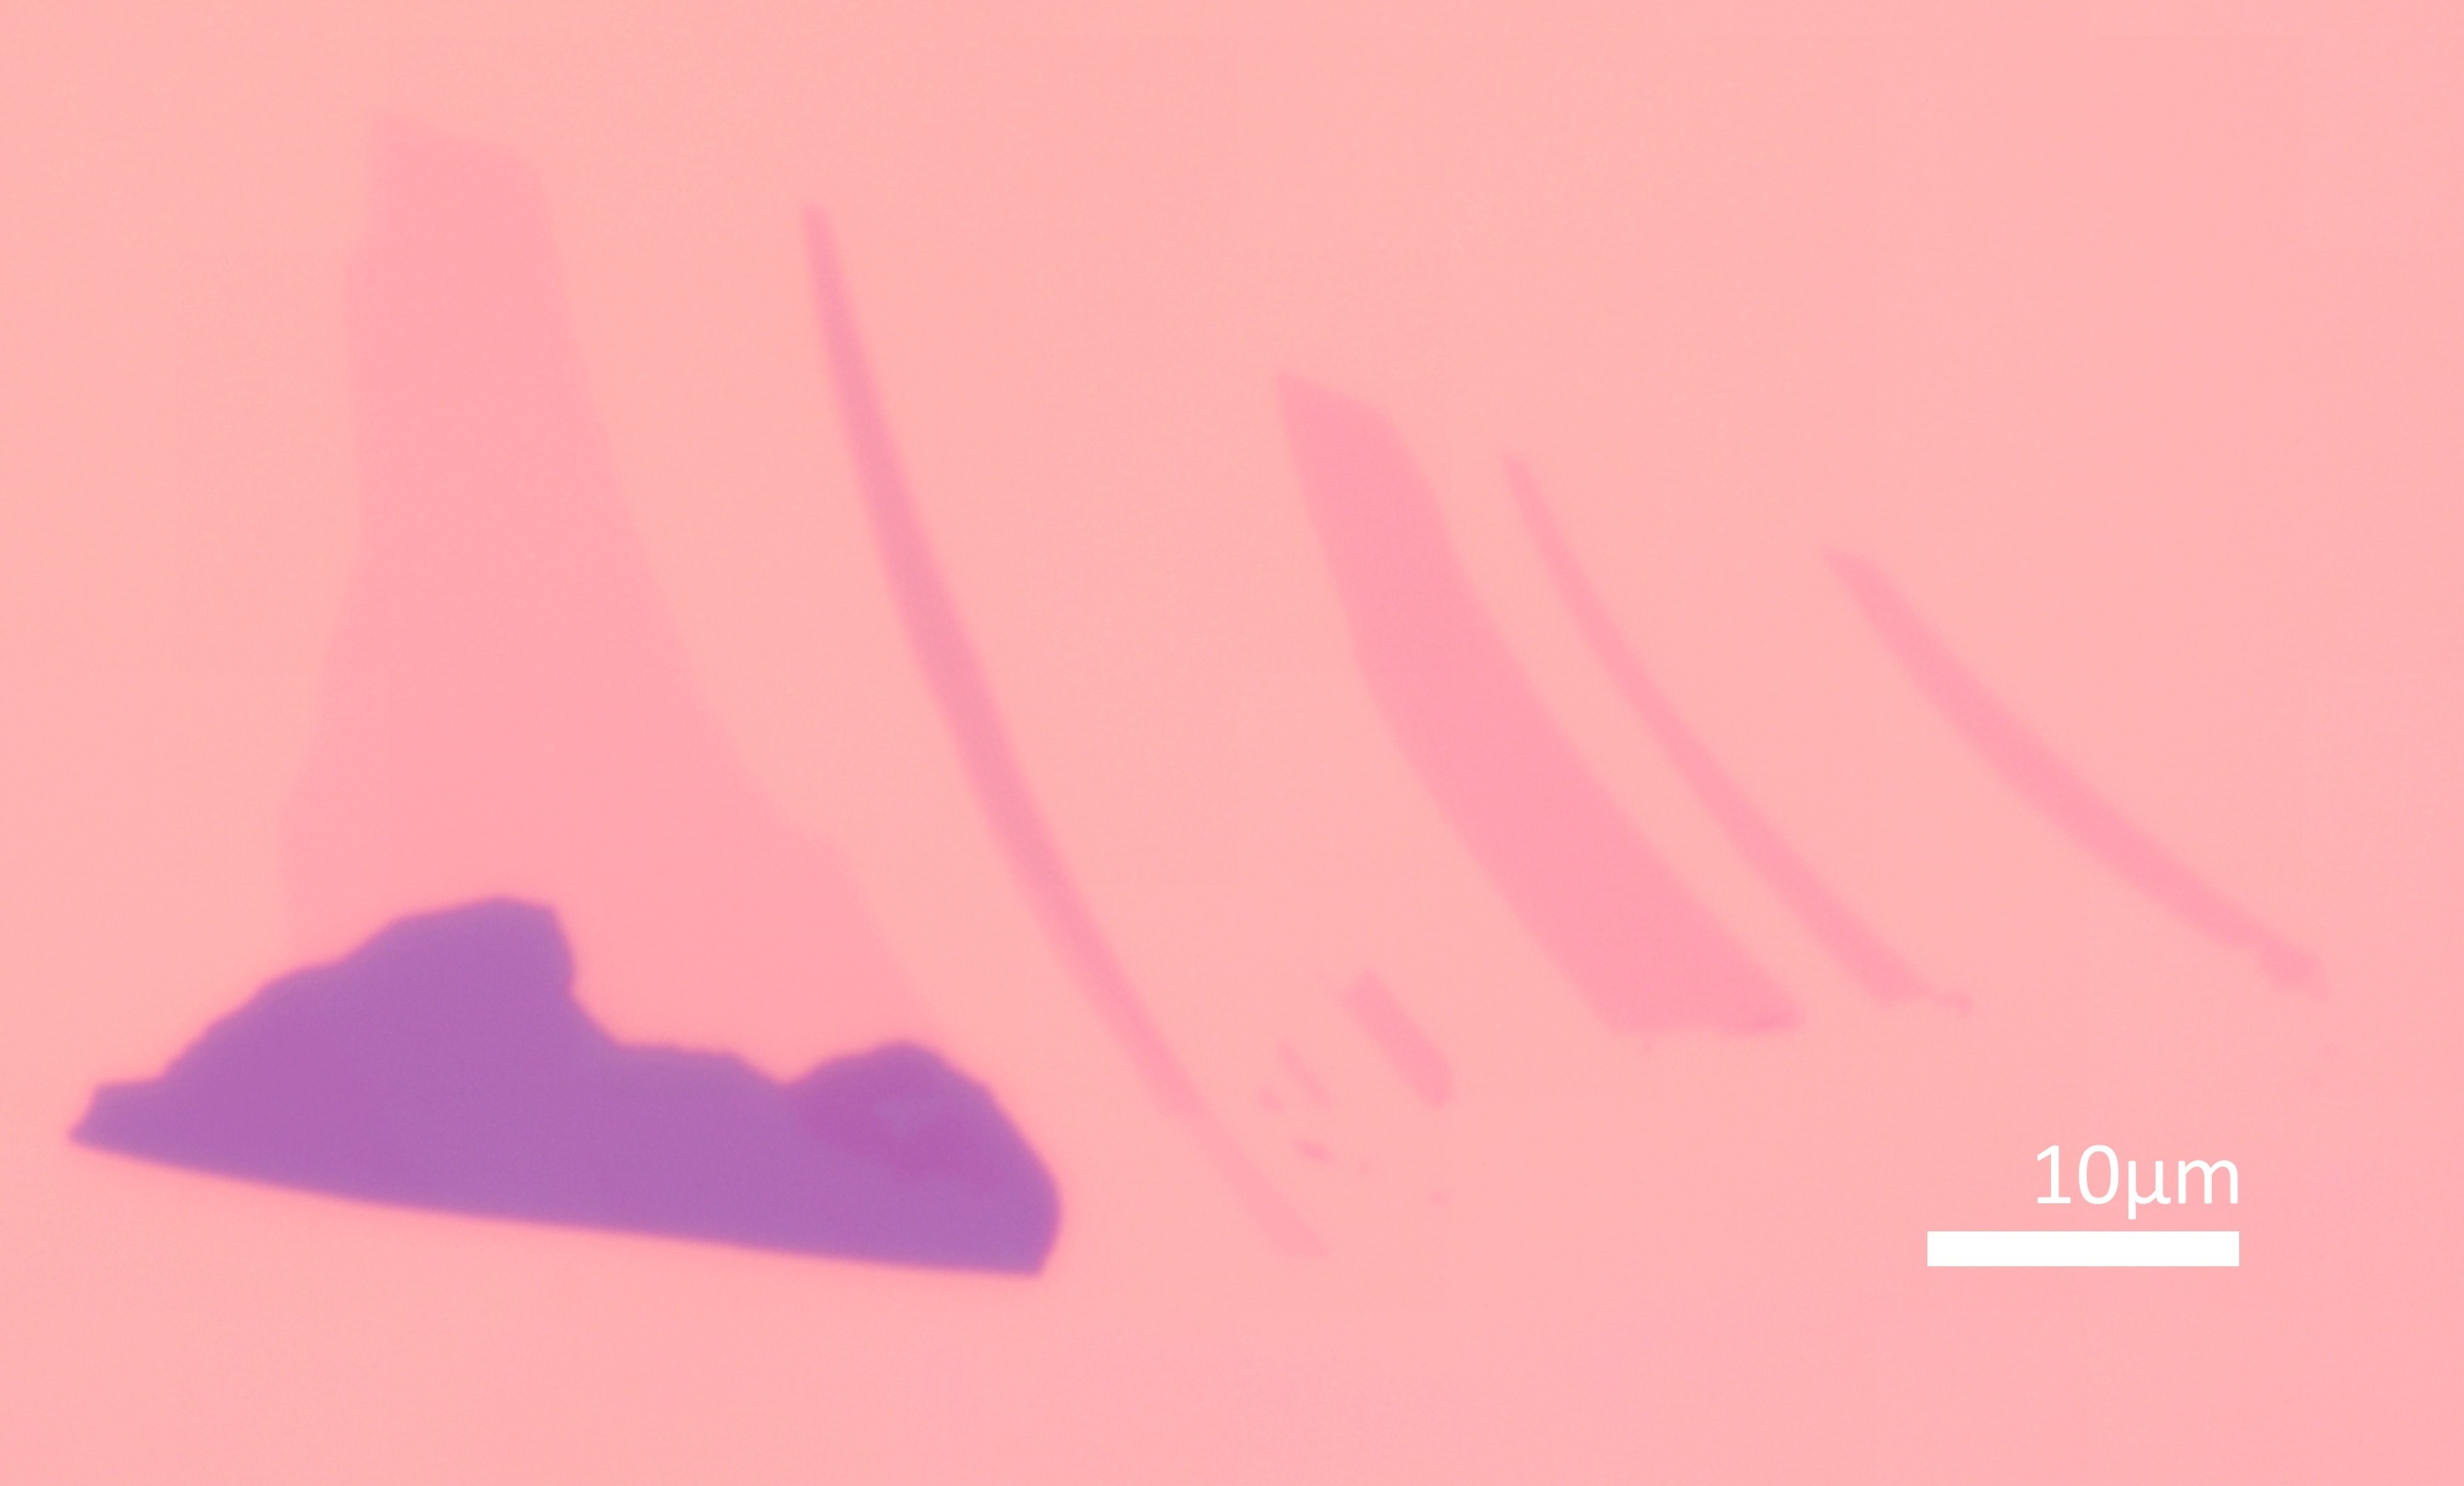
\includegraphics[width=\textwidth]{chap3/raman_contrast1/100x}
%		\caption{100x microscope image}
%	\end{subfigure}
	\begin{subfigure}{\textwidth}
		\includegraphics[width=0.5\textwidth]{chap3/raman_contrast1/raman_spectrum_graphene}
		\includegraphics[width=0.5\textwidth]{chap3/b4w6f3/raman_spectrum_graphene}
		\caption{Graphene Raman spectrum. The 2D peak is roughly 2x the amplitude of the G peak.}
	\end{subfigure}
	\begin{subfigure}{\textwidth}
		\includegraphics[width=0.5\textwidth]{chap3/raman_contrast1/raman_spectrum_bilayer}
		\includegraphics[width=0.5\textwidth]{chap3/b4w6f3/raman_spectrum_bilayer}
		\caption{Bilayer graphene Raman spectrum. Broader 2D peak that is $\approx\frac{3}{4}$ of the amplitude of the G peak.}
	\end{subfigure}
	\caption[Ratio of G to 2D peaks in graphene and bilayer]{Ratio of G to 2D Peaks in various levels of graphene}\label{fig:raman_data_1}
\end{figure}

Secondly, the 2D peak slowly shifts right and broadens as layers increase. This is distinguishable between a single layer, two layers and multiple layers. For a single layer, the peak fits very well to a single resonance lorentzian. For two layers, 4 lorentz peaks are used to fit the broader 2D resonance.

\begin{figure}[H]
	%	\begin{subfigure}{0.3\textwidth}
	%		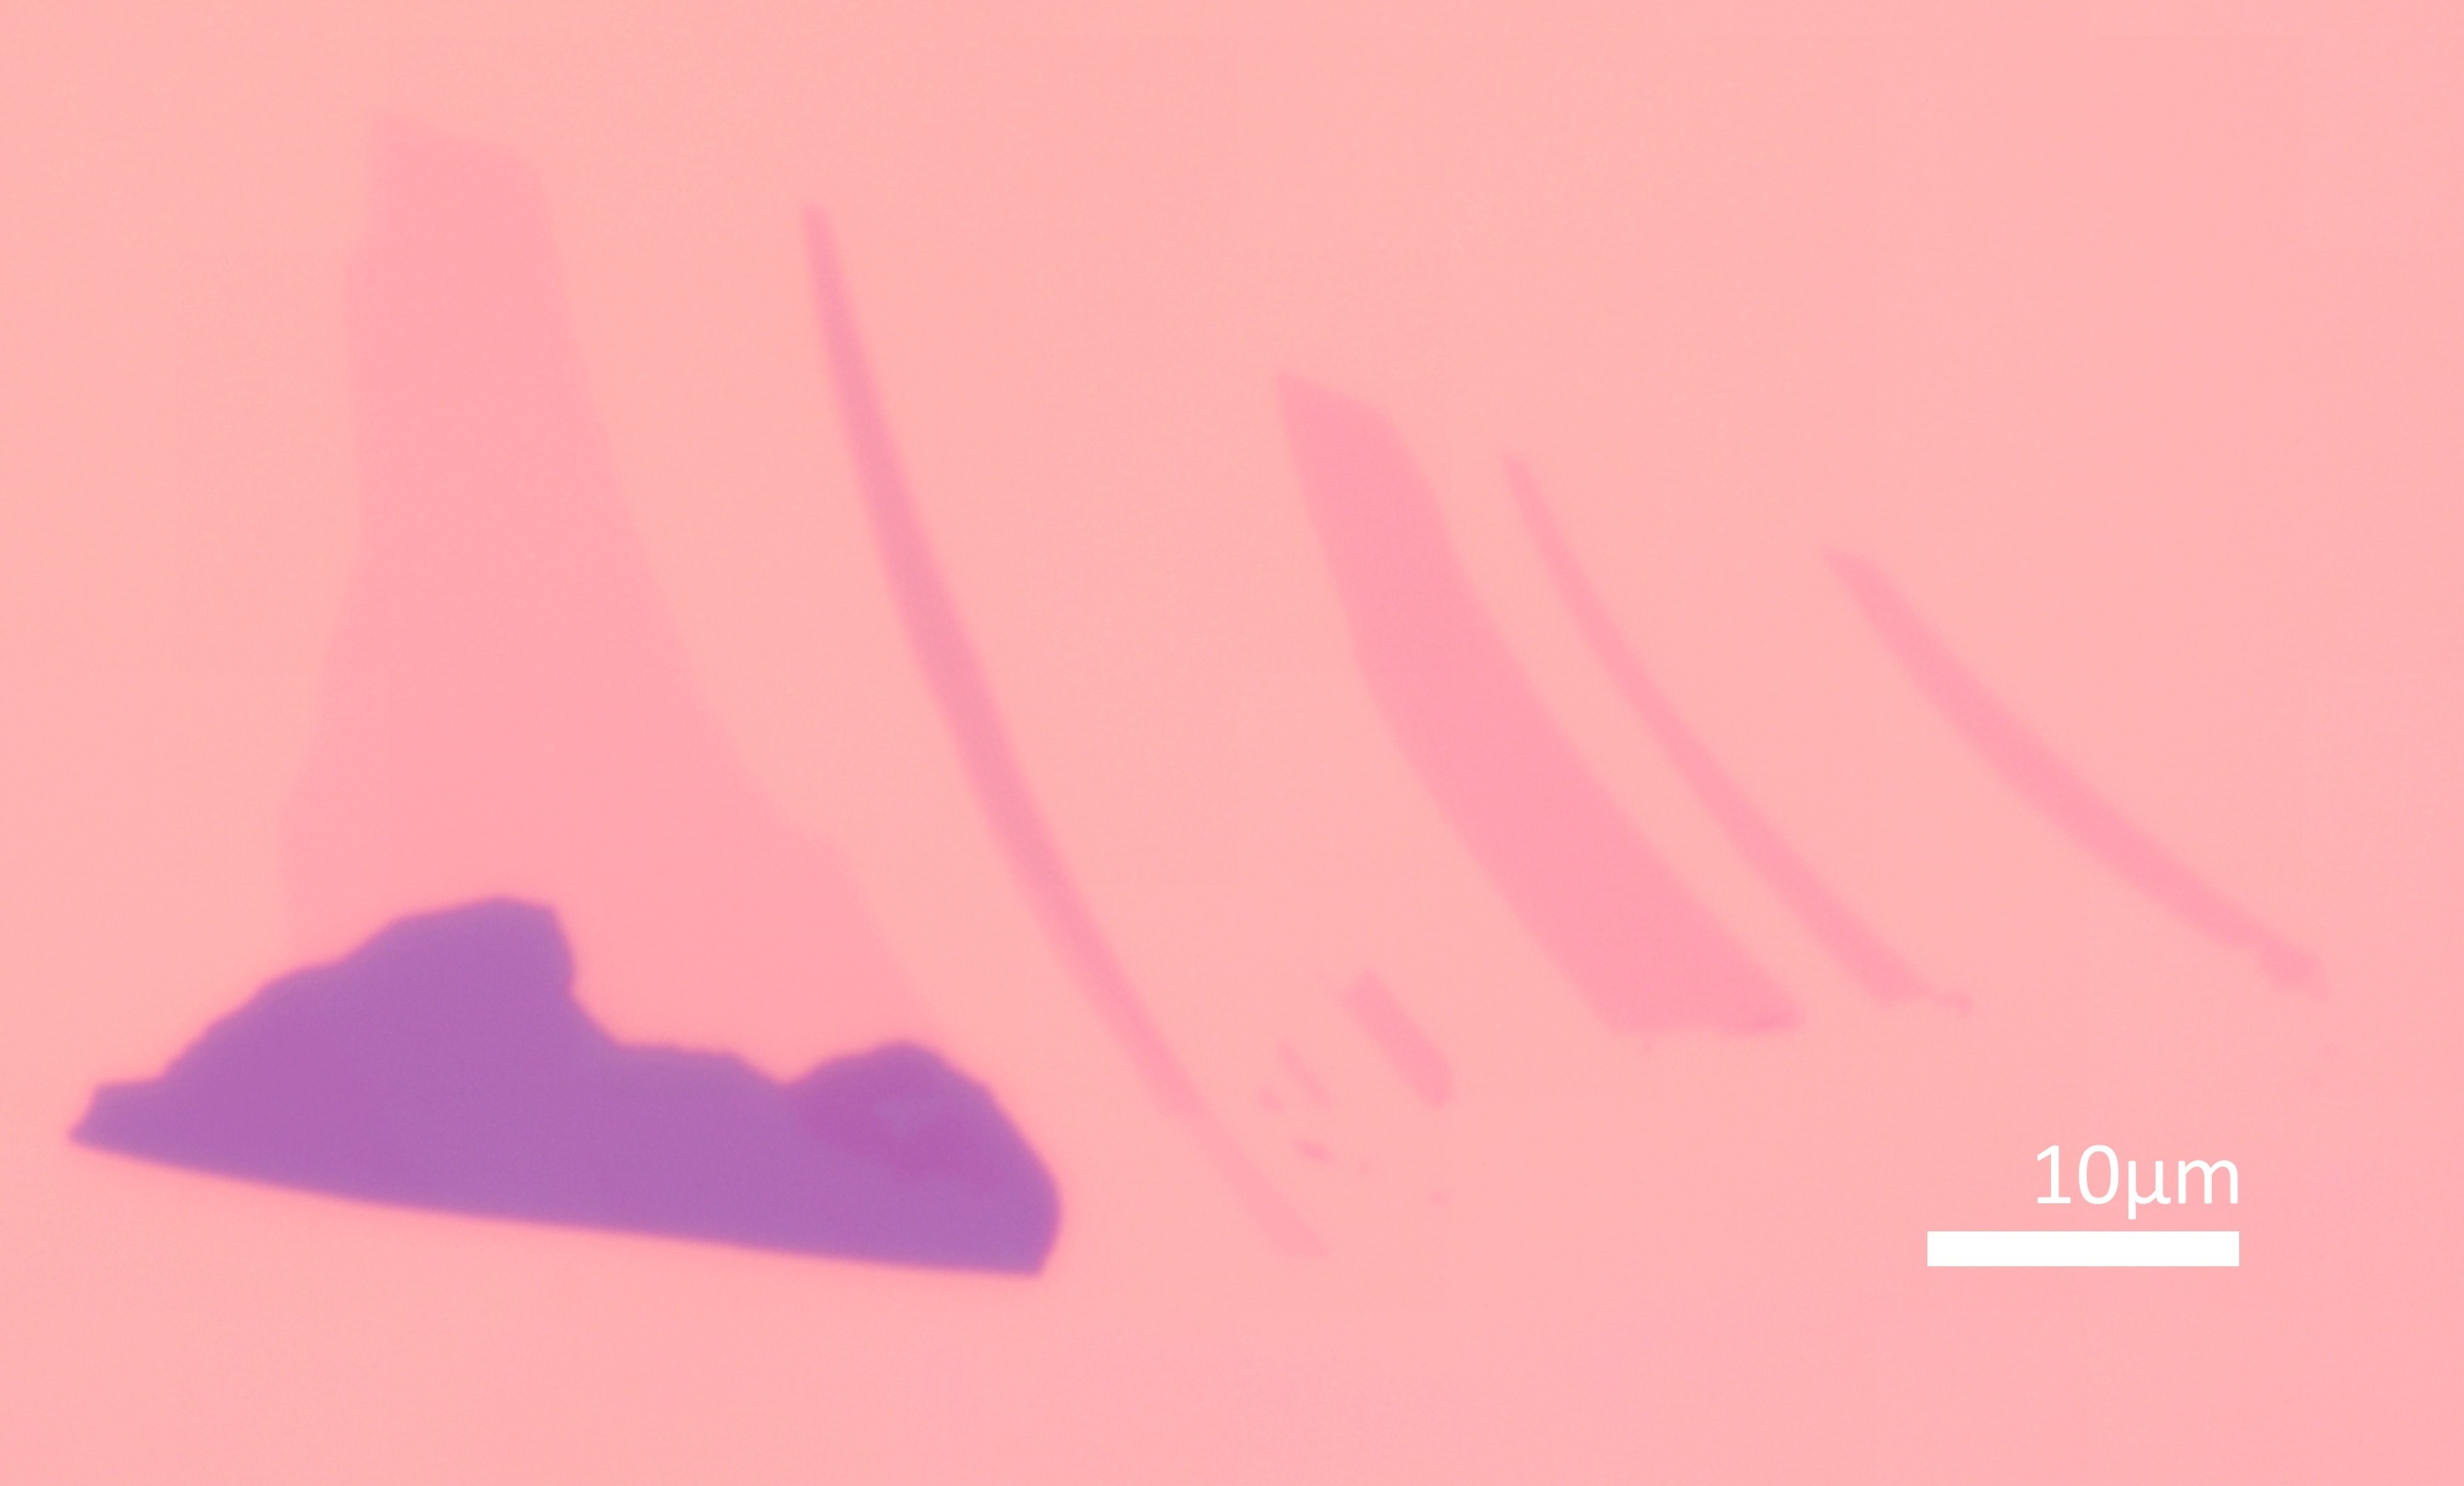
\includegraphics[width=\textwidth]{chap3/raman_contrast1/100x}
	%		\caption{100x microscope image}
	%	\end{subfigure}
	\begin{subfigure}{\textwidth}
		\includegraphics[width=0.5\textwidth]{chap3/raman_contrast1/raman_2dpeak_graphene}
		\includegraphics[width=0.5\textwidth]{chap3/b4w6f3/raman_2dpeak_graphene}
		\caption{Graphene Raman 2D peak.}
	\end{subfigure}
\end{figure}
\begin{figure}[H]
	\ContinuedFloat
	\begin{subfigure}{\textwidth}
		\includegraphics[width=0.5\textwidth]{chap3/raman_contrast1/raman_2dpeak_bilayer}
		\includegraphics[width=0.5\textwidth]{chap3/b4w6f3/raman_2dpeak_bilayer}
		\caption{Bilayer graphene Raman 2D peak.}
	\end{subfigure}
	\caption{Raman 2D fitting of graphene and bilayer}\label{fig:raman_data_2}
\end{figure}

The theoretical picture is quite intuitive for the broadening of the 2D peak seen in \cref{fig:raman_data_2}. Because the 2D peak relates to disorder, and not directly a mode of geometric structure of graphene, the 2D peak is coupled to the electronic structure of graphene (see \cref{fig:raman_graphene}). A single layer of graphene has two bands that meet at dirac points (see \cref{sec:electronic_dispersion}), which allows singular transitions in the momentum/energy profile. A bilayer of graphene has two extra non-degenerate bands instead, allowing a possibility of 4 slightly different transitions near the same energy/momentum profile, contributing to the broadness seen in the Raman spectrum.
\begin{figure}[H]
	\vspace{-0.5cm}
	\begin{subfigure}[t]{0.6\textwidth}
		\centering
		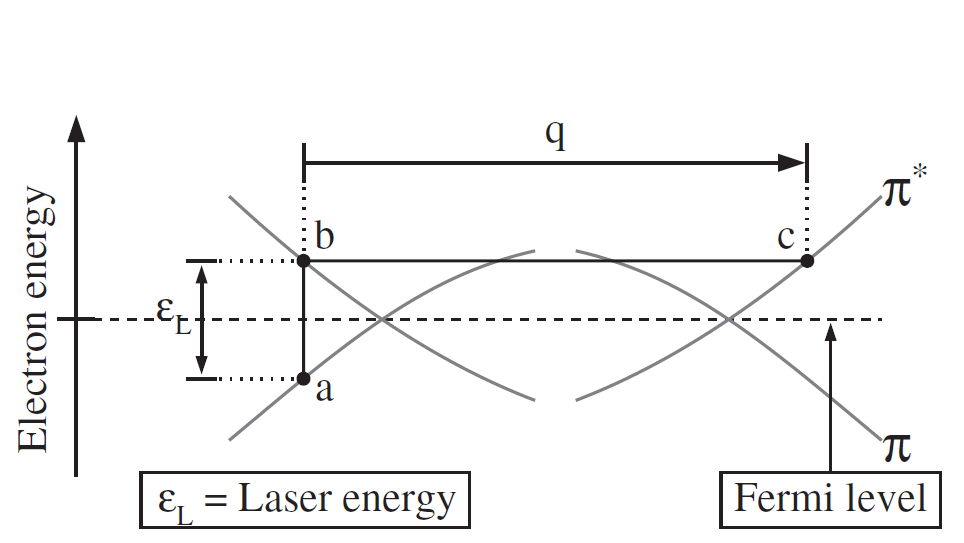
\includegraphics[width=\textwidth]{chap3/Raman_monolayer}
		\caption{Monolayer graphene - One distinct scattering process}
	\end{subfigure}
	\begin{subfigure}[t]{0.4\textwidth}
		\centering
		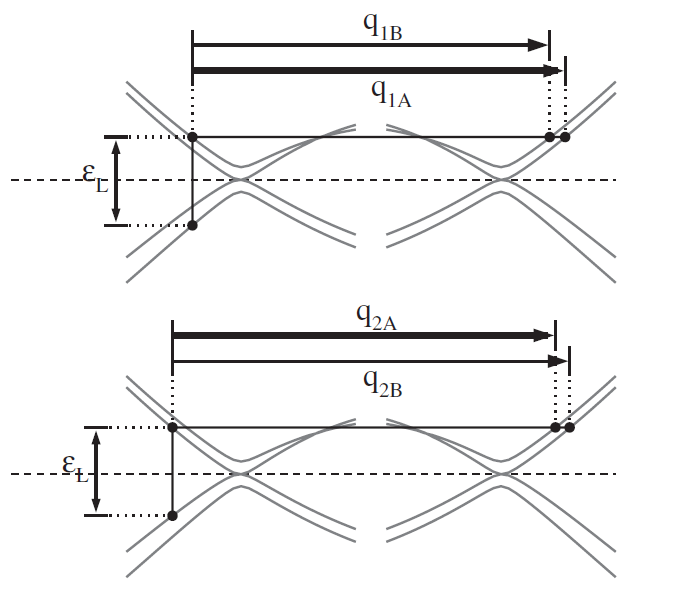
\includegraphics[width=\textwidth]{chap3/Raman_bilayer}
		\caption{Bilayer graphene - Four distinct scattering process}
	\end{subfigure}
	\caption[Raman processes in graphene]{Raman scattering processes in graphene and bilayer graphene, coupled to the electronic structure. Each transition results in a unique change of momentum and energy. \\(Source: Ferrari \etal. \cite{ferrari_raman_2006})}\label{fig:raman_graphene}
\end{figure}

\section{Optical microscopy}
Under a microscope graphene can be optically observed on particular substrates. Blake \etal{.} has studied the optimal wavelengths in which to observe graphene, based on the oxide thickness (SiO$_2$) \cite{blake_making_2007}. We use 285 nm \silicondioxide{} on top of Si to make graphene most pronounced in green wavelengths, which is also the most sensitive colour to the human eye (see \cref{fig:rgb}). A consequence of this strong contrast is that monolayer graphene can be optically identified without the need for more other measurements such as Raman or atomic force microscopy \cite{li_rapid_2013,wang_thickness_2012}. 
\begin{figure}
	\centering
	\begin{subfigure}{0.48\textwidth}
		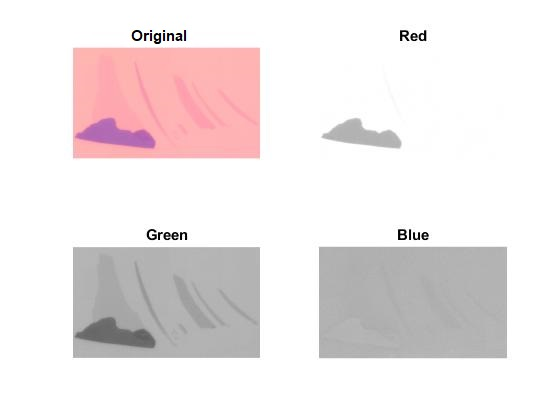
\includegraphics[width=\textwidth]{chap3/B04_W03_F02_RGB}
	\end{subfigure}
	\begin{subfigure}{0.48\textwidth}
		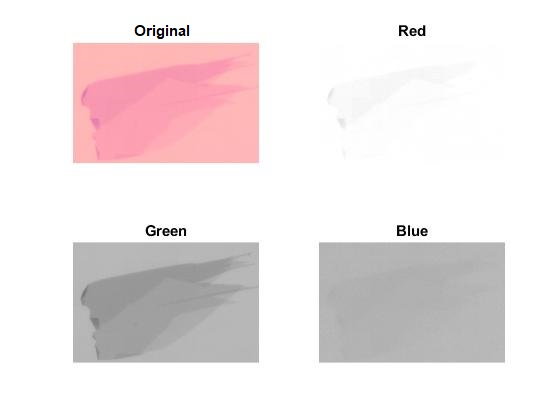
\includegraphics[width=\textwidth]{chap3/B04_W06_F03_RGB}
	\end{subfigure}
	\caption[RGB images of graphene on 285nm \silicondioxide{}]{RGB decomposition of optical images of graphene on 285nm \silicondioxide{}. Most contrast for single or few layers of graphene comes from the green component as desired.}\label{fig:rgb}
\end{figure}
\subsection{Contrast imaging}
Graphene absorbs 2.3\%, passing $\approx$97.7\%, of the light incident on it. This opacity is actually defined by the fine structure constant, physically determined by fundamental quantities \cite{nair_fine_2008}. The fine structure constant describes the fundamental electromagnetic interaction strength of particles. This opacity is one of the few phenomena in condensed matter physics that doesn't depend on material parameters, and is pretty spectacular (excuse the optical pun) to consider.

Graphene exhibits a universal electrical conductance minimum of $\approx 4 (e^2/h)$ (see \cref{sec:charged_puddling}), and as a result \cite{kuzmenko_universal_2008} the optical conductance is also expected to have a fundamental value, behaving independent of frequency (to a broad range of photon energies). This uniform frequency response is due to the linearity of the electronic band structure around the dirac points, which phonons interact with.
\begin{align}
	\alpha&= \frac{\pi e^2}{\hbar c} \approx \frac{1}{137}\\
	\pi \alpha &\approx 2.3\%
\end{align}

We can use this property of graphene's optical transmittance to perform contrast imaging of graphene, identifying single layers from the contrast between the substrate beneath and the flake of interest.  \cite{li_rapid_2013,wang_thickness_2012,ni_graphene_2007} 

If light passes from a source through the graphene, reflecting from the \silicondioxide{} and passing back through the graphene, then we expect approximately 5\% absorbtion of our incident intensity, which will cause a contrast change.
We calculate a contrast value for each pixel by using the green pixel value of each square $\left(G\in[0,1]\right)$ and taking the difference from the background mode $G_0$. \cite{ni_graphene_2007,wang_thickness_2012} Dividing by the background mode gives a percentage change.
\begin{align}
C = \frac{G-G_0}{G_0}\label{eqn:contrast}
\end{align}
This contrast formula takes a green colourvalue representing the background contrast, and observes the percentage change when layers of graphene are on top of it. This percentage absorbtion should roughly match the expected 2.33\% per transmission through graphene, as the pixel value approaches black (value $G=0$) with more layers.

\Cref{fig:contrast1} and \cref{fig:contrast2} both clearly indicate peaks for single layers near 6\% contrast, and multiples of that for larger layers. This is a little higher than expected, but given RGB capture is 0-255, the uncertainty in pixel capture is roughly $1/255 \approx 0.4\%$ making this deviation reasonable.
\begin{figure}[H]
	\centering
	\begin{subfigure}[b]{0.6\textwidth}
		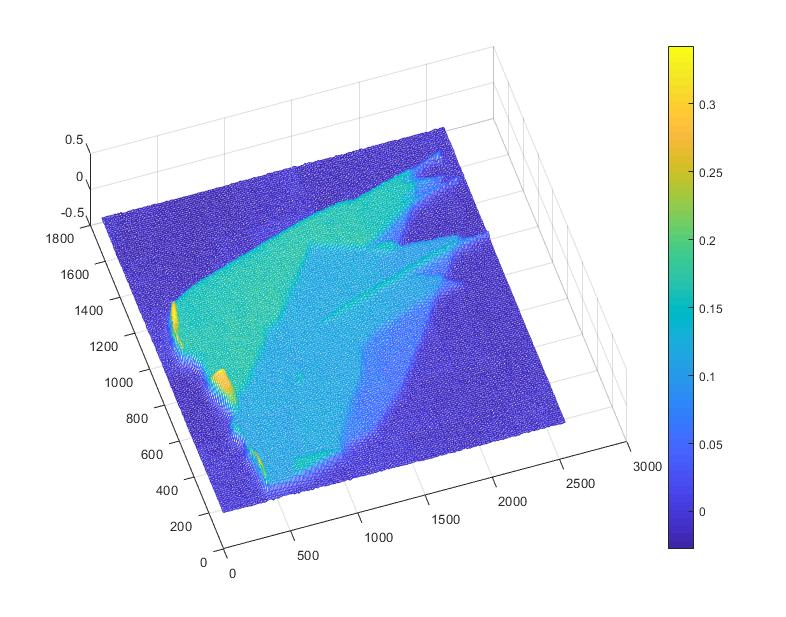
\includegraphics[width=\textwidth]{chap3/B04_W06_F03_mesh2}
		\caption{Contrast surface}
	\end{subfigure}
	\begin{subfigure}[b]{0.35\textwidth}
		\centering
		\begin{subfigure}{\textwidth}
			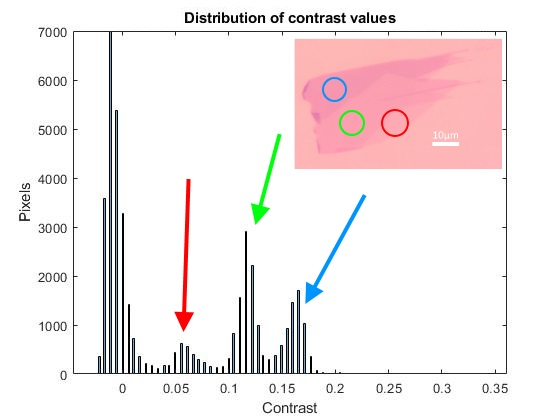
\includegraphics[width=\textwidth]{chap3/B04_W06_F03_histogram_v2}
			\caption{Histogram of contrast values}
		\end{subfigure}\\
		\begin{subfigure}{\textwidth}
			\centering
			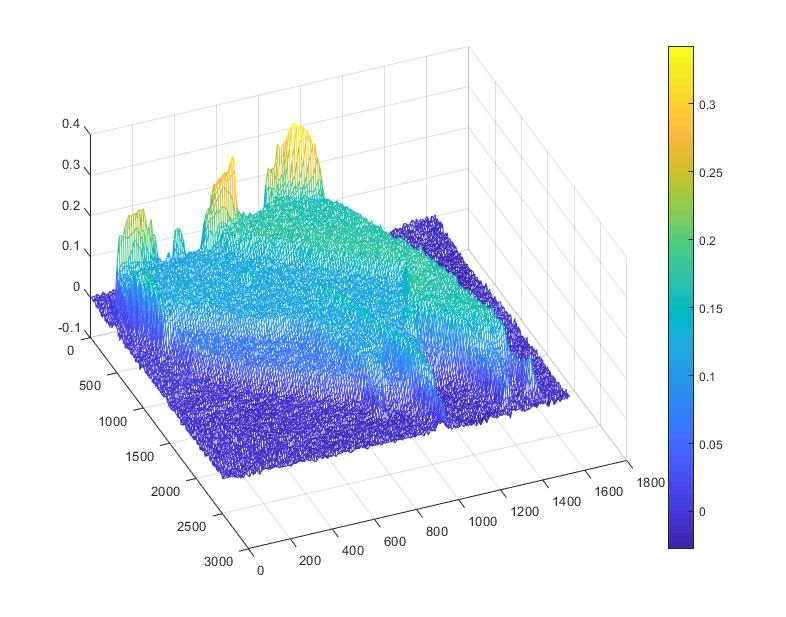
\includegraphics[width=0.85\textwidth]{chap3/B04_W06_F03_mesh4}
		\end{subfigure}
		\caption{Alternative angle}
	\end{subfigure}
	\caption[Contrast imaging sample 1]{Contrast imaging of sample 1.}\label{fig:contrast1}
\end{figure}
\begin{figure}[H]
	\centering
	\begin{subfigure}[b]{0.6\textwidth}
		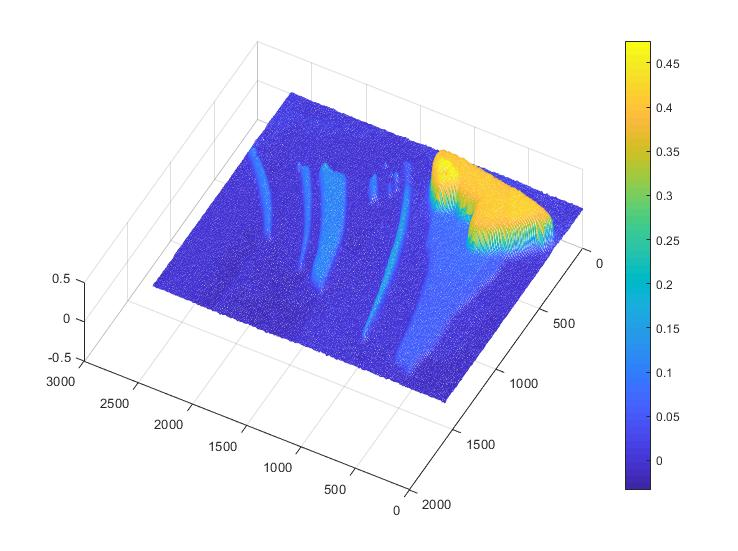
\includegraphics[width=\textwidth]{chap3/B04_W03_F02_mesh1}
		\caption{Contrast surface}
	\end{subfigure}
	\begin{subfigure}[b]{0.35\textwidth}
		\centering
		\begin{subfigure}{\textwidth}
			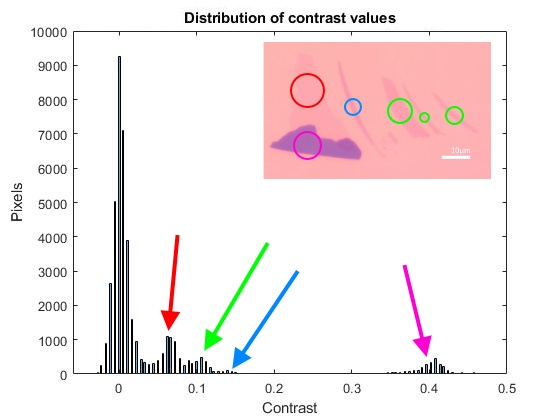
\includegraphics[width=\textwidth]{chap3/B04_W03_F02_histogram_v2}
			\caption{Histogram of contrast values}
		\end{subfigure}\\
		\begin{subfigure}{\textwidth}
			\centering
			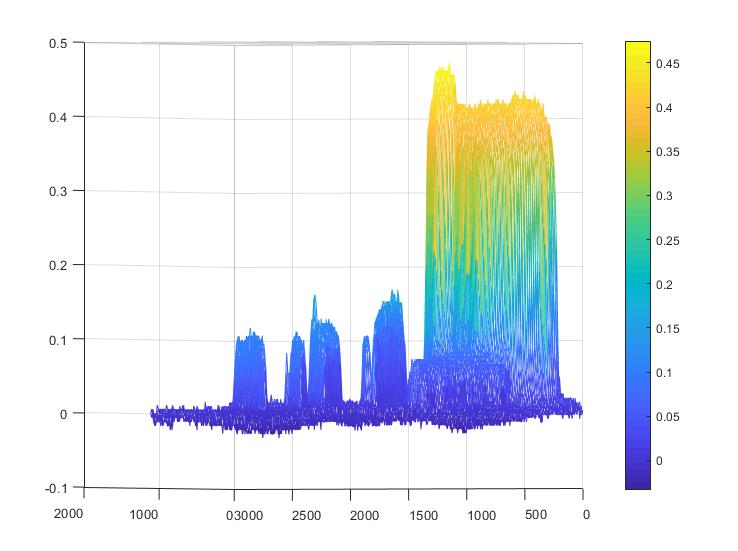
\includegraphics[width=0.85\textwidth]{chap3/B04_W03_F02_mesh2}
		\end{subfigure}
		\caption{Alternative angle}
	\end{subfigure}
	\caption[Contrast imaging sample 2]{Contrast imaging of sample 2.}\label{fig:contrast2}
\end{figure}
%\section{Atomic force microscopy}
%TODO AFM if you have all the time in the world...
\end{document}